
\lecture{Point Estimates}{point-estimates}
\section{Point Estimates}

\title{Point Estimates}
\subtitle{Estimating Parameters}

%\author{Kelly Black}
%\institute{Clarkson University}
\date{18 October 2013}

\begin{frame}
  \titlepage
\end{frame}

\begin{frame}
  \frametitle{Outline}
  \tableofcontents[hideothersubsections,sectionstyle=show/hide]
\end{frame}


\iftoggle{clicker}{%
  \subsection{Clicker Question}
  \begin{frame}
    \frametitle{Find The Sample mean}
    (Use channel 42)

    \vfill 
    
    \begin{tabular}{lll}
      3, & 5, & -2
    \end{tabular}

    \vfill

    \begin{tabular}{l@{\hspace{3em}}l@{\hspace{3em}}l}
      a: -2 & b: 2 & c: 4
    \end{tabular}

    \vfill


  \end{frame}
}


\subsection{Point Estimates}

\begin{frame}{Point Estimates}

  We have a random variables and have samples of the random
  variable:\\ [10pt]
  \begin{tabular}{l|l}
    Observation & Value \\ \hline
    1 & $x_1$ \\ 
    2 & $x_2$ \\
    3 & $x_3$ \\
    \vdots & \vdots \\
    $n$ & $x_n$
  \end{tabular}

  \vfill

  What estimate can we make for a ``parameter?''

  \vfill
  
\end{frame}


\begin{frame}{Parameters versus Statistic}

  \begin{definition}[Parameter]
    A \redText{parameter} is a quantity that is a \blueText{property}
    of the random variable.
  \end{definition}

  \begin{definition}[Statistic]
    A \redText{statistic} is a \blueText{calculation} based on a set
    of samples.
  \end{definition}

\end{frame}




\begin{frame}
  \frametitle{Example}

  A random variable has a mean $\mu$ and standard deviation
  $\sigma$. A set of samples is taken: \\ [10pt]
  \begin{tabular}{l|l}
    Observation & Value \\ \hline
    1 & $1.0$ \\ 
    2 & $3.0$ \\
    3 & $8.0$ \\
    4 & $4.0$ \\
    5 & $7.0$
  \end{tabular}

\end{frame}


\begin{frame}{Point Estimate}

  \begin{definition}[Point Estimate]
    A \redText{point estimate} is an \blueText{estimate} of a
    parameter based on whatever, limited, information that is
    available to us.
  \end{definition}
\end{frame}


\begin{frame}{Example}

  $\bar{x}$ is an estimate for the mean.
  
\end{frame}

\begin{frame}{Example}
  How likely is it that a coin flip returns a tails?

  \vfill

  Flip a coin seven times.

  \vfill

\end{frame}


\begin{frame}{Example}

  The voltage difference across a resistor is measured at random
  times: \\ [10pt]
  \begin{tabular}{l|l}
    Observation & Voltage \\ \hline
    1 & 3.50 \\
    2 & 3.61 \\
    3 & 3.53 \\
    4 & 3.55 
  \end{tabular}
  
\end{frame}

\begin{frame}{Extra Examples}

  \vfill

  The following examples are extra examples that are not covered in
  class.

  \vfill
  
\end{frame}

\begin{frame}{Example}

  \begin{tabular}{lllllll}
    30 & 28 & 31 & 33 & 35 & 22 & 31
  \end{tabular}

  The sample mean:
  \begin{eqnarray*}
    \bar{x} & = & \frac{30 + 28 + 31 + 33 + 35 + 22 + 31}{7}, \\
    & = & 30.
  \end{eqnarray*}

  To get the median first order the data: \\
  \only<1>%
  {
    \begin{tabular}{lllllll}
      22 & 28 & 30 & 31 & 31 & 33 & 35
    \end{tabular}
  }

  \only<2>%
  {
    \begin{tabular}{lllllll}
      {\color{red}22} & {\color{red}28} & {\color{red}30} & 31 & {\color{blue}31} & {\color{blue}33} & {\color{blue}35}
    \end{tabular}
  }

  \only<3->%
  {
    \begin{tabular}{lllllll}
      {\color{red}22} & {\color{red}28} & {\color{red}30} & $\underbrace{31}_{Median}$ & {\color{blue}31} & {\color{blue}33} & {\color{blue}35}
    \end{tabular}
  }
  
\end{frame}


\begin{frame}{Example}

  Even number of data points.

  \begin{tabular}{lllllll}
    30 & 28 & 31 & 33 & 35 & 22 
  \end{tabular}

  The sample mean:
  \begin{eqnarray*}
    \bar{x} & = & \frac{30 + 28 + 31 + 33 + 35 + 22}{6}, \\
    & = & 29.8.
  \end{eqnarray*}

  To get the median first order the data: \\
  \only<1>%
  {
    \begin{tabular}{llllll}
      22 & 28 & 30 & 31 & 33 & 35
    \end{tabular}
  }

  \only<2>%
  {
    \begin{tabular}{llllll}
      {\color{red}22} & {\color{red}28} & 30 & 31  & {\color{blue}33} & {\color{blue}35}
    \end{tabular}
  }

  \only<3->%
  {
    \begin{tabular}{llccll}
      {\color{red}22} & {\color{red}28} & 30 & 31 & 
      {\color{blue}33} & {\color{blue}35} \\
      & & \multicolumn{2}{c}{Median = $\frac{30+31}{2}$} 
    \end{tabular}
  }
  
\end{frame}


\begin{frame}
  \frametitle{Clicker Quiz}
  (Use channel 42)

  Find the median of the following data set:
  \vfill 

  \begin{tabular}{llll}
    3, & 5, & 2, & 4
  \end{tabular}

  \vfill

  \begin{tabular}{l@{\hspace{3em}}l@{\hspace{3em}}l@{\hspace{3em}}l}
    a: 5/2  & b: 7/2 & c: 3 & D: 4
  \end{tabular}

  \vfill

  

\end{frame}

\begin{frame}{Why Two Measures?}

  \begin{enumerate}
  \item They represent different things.
  \item The median is more robust.
  \end{enumerate}

  \only<1-2>%
  {
    Example: \\
    \begin{tabular}{llllll}
      94 & 105 & 95 & 97  & 99 & 101
    \end{tabular}

    \only<2>%
    {
      The median is 98, and the mean is 98.5.
    }
  }

  \only<3-4>%
  {
    Alter the example: \\
    \begin{tabular}{llllll}
      94 & 105 & 95 & 97  & 99 & {\color{red}110}
    \end{tabular}

    \only<4>%
    {
      The median is 98, and the mean is 101.7. The median is less
      likely to be altered by outliers.
    }
  }

  
  
\end{frame}

\subsection{Skew}

\begin{frame}{Skew}

  \begin{definition}[Left Skew]
    If the mean is to the left of the median the data is skewed to the
    left.
  \end{definition}

  \begin{definition}[Right Skew]
    If the mean is to the right of the median the data is skewed to
    the right.
  \end{definition}

  \begin{definition}[Symmetric]
    If the mean is close to the median the data is symmetric.
  \end{definition}
  
\end{frame}

\begin{frame}{Skewed to the Left}

  \only<1>%
  {
    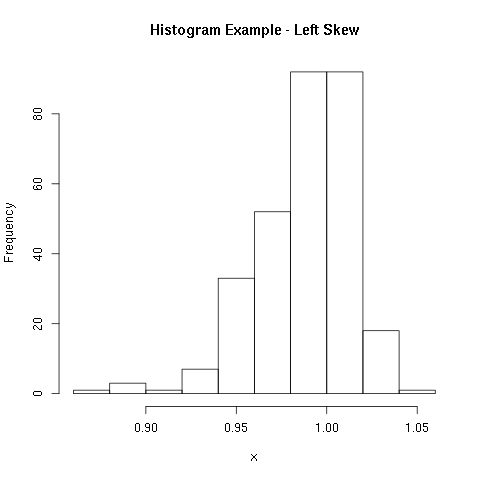
\includegraphics[width=7cm]{img/leftSkew}
  }

  \only<2>%
  {
    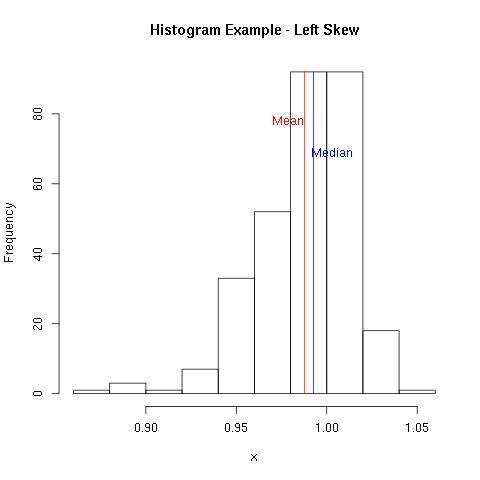
\includegraphics[width=7cm]{img/leftSkewAnnotated}
  }

  
\end{frame}


\begin{frame}{Skewed to the Right}

  \only<1>%
  {
    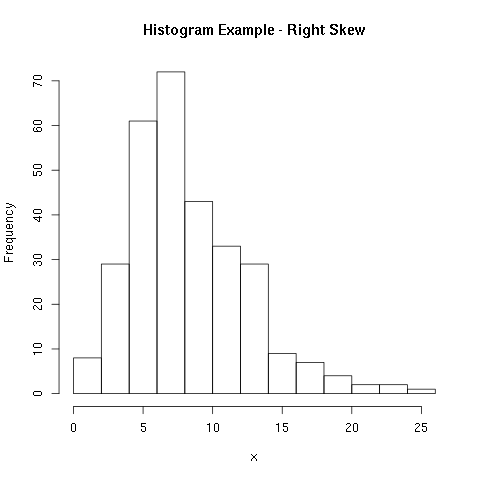
\includegraphics[width=7cm]{img/rightSkew}
  }

  \only<2>%
  {
    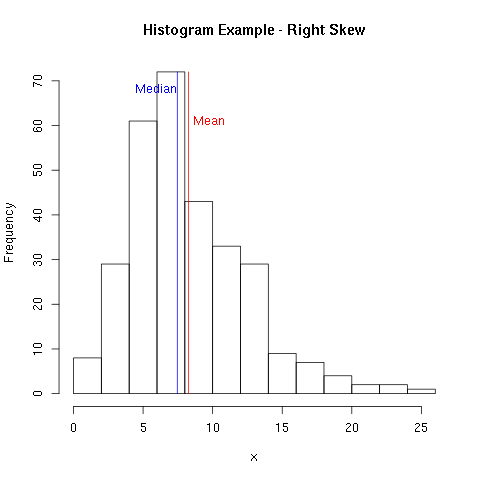
\includegraphics[width=7cm]{img/rightSkewAnnotated}
  }

  
\end{frame}


\begin{frame}{Symmetric}

  \only<1>%
  {
    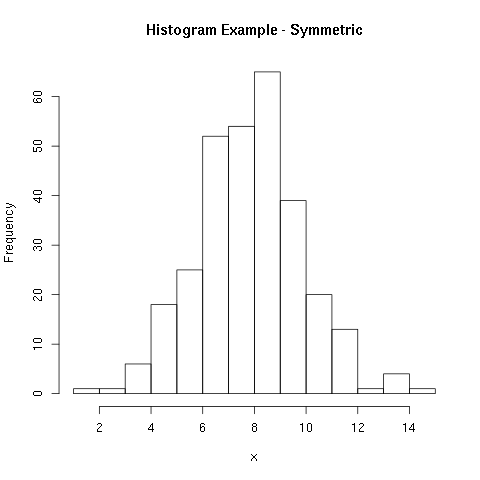
\includegraphics[width=7cm]{img/symmetric}
  }

  \only<2>%
  {
    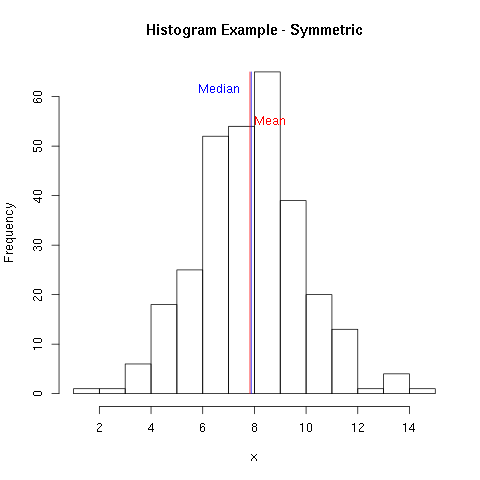
\includegraphics[width=7cm]{img/symmetricAnnotated}
  }

  
\end{frame}



\iftoggle{clicker}{%
  \begin{frame}
    \frametitle{Clicker Quiz}
    (Use channel 42)

    Find the standard deviation of the following data set:
    \vfill 

    \begin{tabular}{llll}
      3, & 3, & 2, & 4
    \end{tabular}

    \vfill

    \begin{tabular}{l@{\hspace{3em}}l@{\hspace{3em}}l@{\hspace{3em}}l}
      a: 0.5  & b: 0.667  & C: 0.707 & D: 0.816
    \end{tabular}

    \vfill

  

  \end{frame}
}







% LocalWords:  Clarkson pausesection hideallsubsections
